\documentclass{exam}
\usepackage{amsmath}
\usepackage{pgfplots}
\usepackage{tikz}
\pgfplotsset{compat=1.15}

\begin{document}

\title{Mathematics Mock Exam}
\date{Tag: 987934937}
\maketitle

\section{ARITHMETIC}
\begin{questions}
\question What is the result of $45 + 37$?
\question Calculate the difference between $300$ and $167$.
\question Multiply $23$ by $3$.
\question Divide $72$ by $9$.
\question What is $5$ to the power of $3$?
\end{questions}

\section{NUMBER AND PLACE VALUE}
\begin{questions}
\question Write the number $5073$ in words.
\question What is the value of the digit $5$ in the number $354$?
\question Write $7000 + 500 + 40 + 2$ in standard form.
\question Round the number $7845$ to the nearest thousand.
\question What is the Roman numeral for $50$?
\end{questions}

\section{FRACTIONS}
\begin{questions}
\question Simplify the fraction $\frac{14}{42}$.
\question Add the fractions $\frac{1}{4}$ and $\frac{3}{8}$.
\question Subtract $\frac{2}{3}$ from $\frac{5}{6}$.
\question Multiply $\frac{2}{5}$ by $\frac{3}{4}$.
\question Divide $\frac{3}{4}$ by $\frac{2}{5}$.
\end{questions}

\section{DECIMALS}
\begin{questions}
\question Write $0.75$ as a fraction.
\question Add $2.3$ and $4.67$.
\question Subtract $0.8$ from $3.45$.
\question Multiply $1.2$ by $3.5$.
\question Divide $2.5$ by $0.5$.
\end{questions}

\section{PERCENTAGES}
\begin{questions}
\question Write $45\%$ as a fraction.
\question What is $30\%$ of $200$?
\question Increase $400$ by $15\%$.
\question Decrease $80$ by $25\%$.
\question What percentage of $50$ is $10$?
\end{questions}

\section{MEASUREMENT AND GEOMETRY}
\begin{questions}
\question Calculate the area of a rectangle with length $7$ cm and width $3$ cm.
\question What is the perimeter of a square with side length $4$ cm?
\question Calculate the volume of a cube with edge length $3$ cm.
\question What is the total surface area of a cuboid with dimensions $2$ cm, $3$ cm and $4$ cm?
\question What is the circumference of a circle with a radius of $3$ cm? (Use $\pi \approx 3.14$)
\end{questions}

\section{GRAPHS AND BAR CHARTS}

\paragraph Here is a bar chart of the number of pets in a class. Use it to answer the questions.
\newline
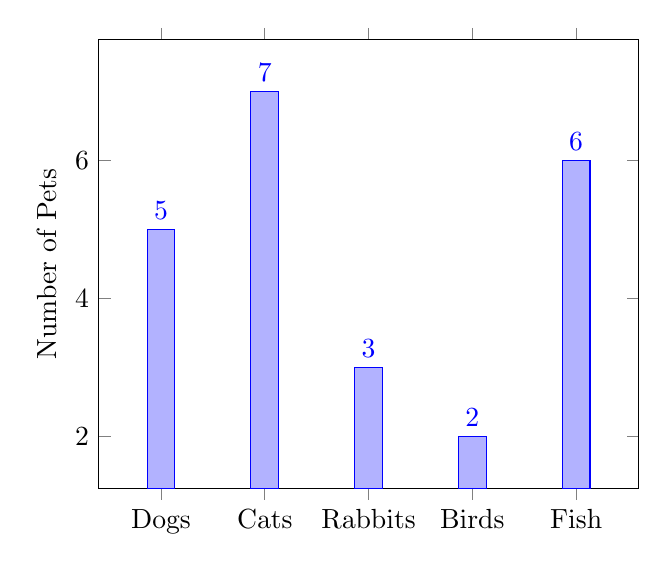
\begin{tikzpicture}
\begin{axis}[
    ybar,
    enlargelimits=0.15,
    ylabel={Number of Pets},
    symbolic x coords={Dogs, Cats, Rabbits, Birds, Fish},
    xtick=data,
    nodes near coords,
    nodes near coords align={vertical},
]
\addplot coordinates {(Dogs,5) (Cats,7) (Rabbits,3) (Birds,2) (Fish,6)};
\end{axis}
\end{tikzpicture}

\begin{questions}
\question How many students have dogs as pets?
\question Which pet is the least popular?
\question How many more students have cats than rabbits?

\end{questions}

\end{document}
